\section{Introduction \& Background}

\subsection{General Introduction}
%%%%%%%%%%%%%%%%%%%%%%%%%%%%%%%%%%   1    %%%%%%%%%%%%%%%%%%%%%%%%%%%%%%% 
\begin{withoutheadline}
\begin{frame}{ General Introduction}


\setbeamercolor{block title}{bg=blue!30,fg=black}
\setbeamercolor{block body}{bg=blue!10,fg=black}
\setbeamertemplate{blocks}[rounded][shadow=false]

\begin{block}{ IoT \& Wireless Sensor Networks}
    \begin{itemize}
    \item Network technologies and IoT. 
    \item<2-> WSN: standardization of IoT nodes communication.
    \item<3-> Main contributions are : low power consumption, low cost.
    \item<4->  IEEE802.15.4 one of the main standards of WSN. 
    \end{itemize}
    \end{block}

 \begin{figure}[p]

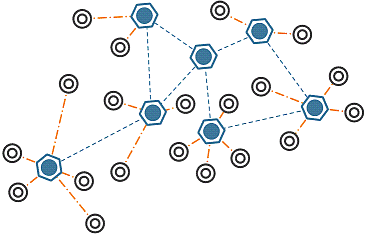
\includegraphics[width=0.5\linewidth]{figures/wsn.png}
  
\end{figure}

\end{frame}
\end{withoutheadline}
%%%%%%%%%%%%%%%%%%%%%%%%%%%%%%%%%%%%%%%%%%%%%%%%%%%%%%%%%%%%%%%%%%%%%%%

\begin{withoutheadline}
\begin{frame}{General intoduction}{IEEE802.15.4}

\setbeamercolor{block title}{bg=blue!30,fg=black}
\setbeamercolor{block body}{bg=blue!10,fg=black}
\setbeamertemplate{blocks}[rounded][shadow=false]


\begin{minipage}[t]{0.48\linewidth}

\begin{block}{Converge Cast Structure}
    \begin{itemize}
    \item Nodes radio ranges defines the neighborhood.
    \item<2-> \alert{Sink} is selected. 
    \item<3-> Packets are forwarded \alert{toward the sink}.
    \item<4-> Communication pairs.
    \end{itemize}
    \end{block}
\end{minipage}\hfill
\begin{minipage}[t]{0.48\linewidth}
\centering
 \begin{figure}[p]

 \only<1>{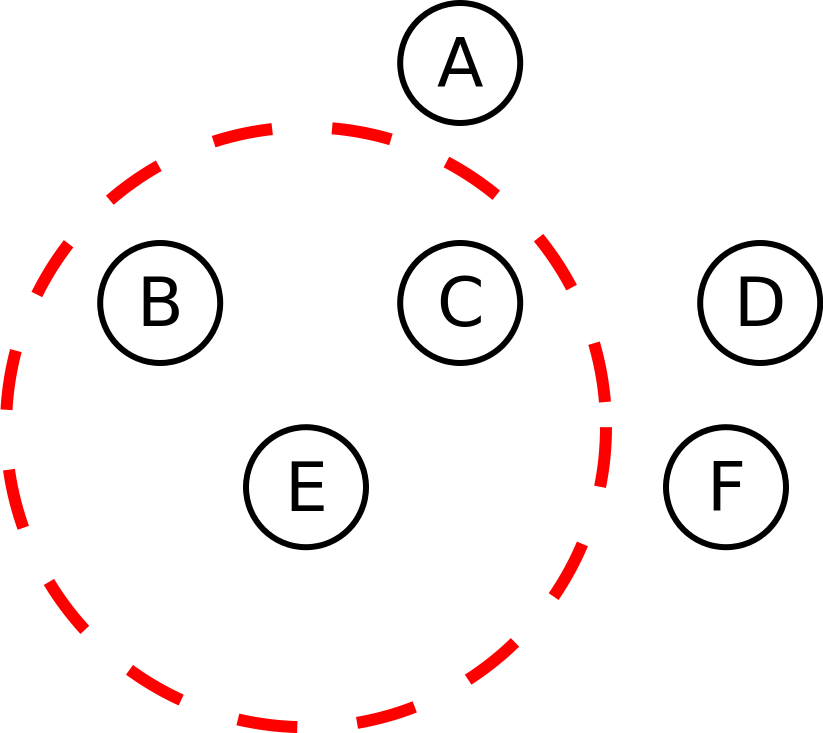
\includegraphics[width=\linewidth]{figures/map1.png}}
  \only<2>{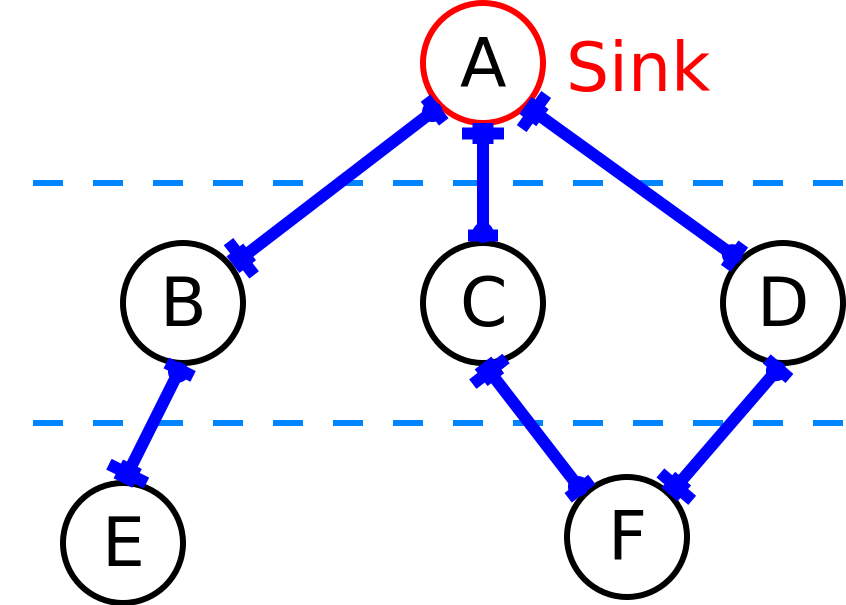
\includegraphics[width=\linewidth]{figures/map2.png}}
  \only<3>{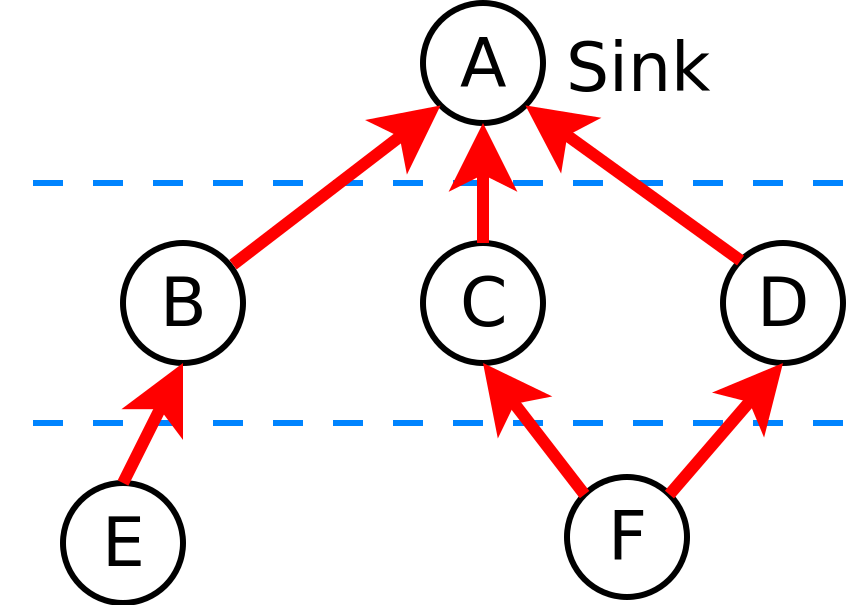
\includegraphics[width=\linewidth]{figures/map3.png}}
  \only<4>{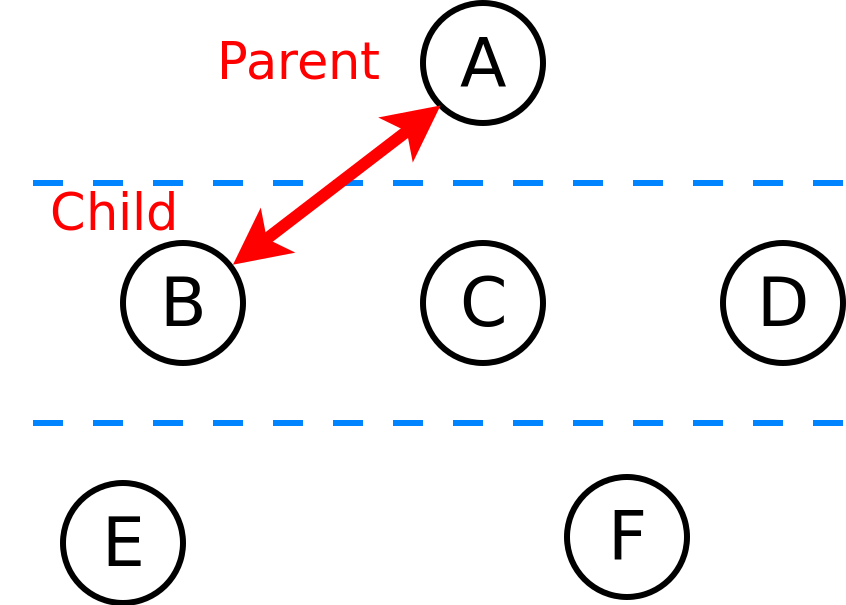
\includegraphics[width=\linewidth]{figures/map4.png}}
  
\end{figure}
\end{minipage}

   
    
    

\end{frame}
\end{withoutheadline}
%%%%%%%%%%%%%%%%%%%%%%%%%%%%%%%%%%%%%%%%%%%%%%%%%%%%%%%%%%%%%%%%%%%%%%%%%%%%%%

\subsection{IEEE802.15.4 Protocols}

\begin{withoutheadline}
\begin{frame}


\setbeamercolor{block title}{bg=blue!30,fg=black}
\setbeamercolor{block body}{bg=blue!10,fg=black}
\setbeamertemplate{blocks}[rounded][shadow=false]




\end{frame}
\end{withoutheadline}

\subsection{Project challenges \& Objectives}


\begin{withoutheadline}
\begin{frame}


\setbeamercolor{block title}{bg=blue!30,fg=black}
\setbeamercolor{block body}{bg=blue!10,fg=black}
\setbeamertemplate{blocks}[rounded][shadow=false]




\end{frame}
\end{withoutheadline}
